\documentclass[11pt,twoside]{book}

\usepackage[T1]{fontenc}
\usepackage[utf8]{inputenc}
\usepackage[paperwidth=6in,paperheight=9in,inner=0.95in,outer=0.65in,top=0.85in,bottom=0.9in,headsep=0.32in]{geometry}
\usepackage{libertine}
\usepackage{microtype}
\usepackage{xcolor}
\usepackage{tikz}
\usetikzlibrary{positioning,calc,shapes.geometric,decorations.pathmorphing}
\usepackage{titlesec}
\usepackage{fancyhdr}
\usepackage{enumitem}
\usepackage[most]{tcolorbox}
\tcbuselibrary{skins}
\usepackage{lettrine}
\usepackage{setspace}

\definecolor{heritageGreen}{HTML}{2F4B3C}
\definecolor{heritageGold}{HTML}{B08D45}
\definecolor{heritageCream}{HTML}{F5EFE3}
\definecolor{heritageCharcoal}{HTML}{2B2622}

\pagecolor{white}
\color{heritageCharcoal}
\setstretch{1.08}

\setlength{\headheight}{14pt}

\newcommand{\ornateRule}{%
  \begin{tikzpicture}[baseline=-0.5ex]
    \draw[heritageGold,line width=0.6pt] (0,0) -- (2.3,0);
    \node[diamond,draw=heritageGold,fill=heritageGold,minimum width=6pt,minimum height=6pt,inner sep=0pt] at (2.55,0) {};
    \draw[heritageGold,line width=0.6pt] (2.8,0) -- (5.1,0);
  \end{tikzpicture}%
}

\newcommand{\smallOrnateRule}{%
  \begin{tikzpicture}[baseline=-0.5ex]
    \draw[heritageGold,line width=0.5pt] (0,0) -- (0.9,0);
    \node[diamond,draw=heritageGold,fill=heritageGold,minimum width=4pt,minimum height=4pt,inner sep=0pt] at (1.05,0) {};
    \draw[heritageGold,line width=0.5pt] (1.2,0) -- (2.1,0);
  \end{tikzpicture}%
}

\titleformat{\chapter}[display]
  {\centering}
  {\normalfont\color{heritageGold}\fontsize{11}{13}\selectfont\MakeUppercase{Chapter \thechapter}}
  {8pt}
  {\ornateRule\\\vspace{12pt}\color{heritageGreen}\normalfont\fontsize{27}{30}\selectfont\scshape}
  [\vspace{6pt}]
\titlespacing*{\chapter}{0pt}{15pt}{34pt}

\renewcommand{\chaptermark}[1]{\markboth{\MakeUppercase{#1}}{}}

\pagestyle{fancy}
\fancyhf{}
\fancyhead[LE]{\small\scshape\color{heritageCharcoal}\leftmark}
\fancyhead[RO]{\small\scshape\color{heritageCharcoal}The Chronicles of Nimbus Valley}
\fancyfoot[LE,RO]{\small\color{heritageGold}\thepage}
\renewcommand{\headrulewidth}{0.4pt}
\renewcommand{\headrule}{\hbox to\headwidth{\color{heritageGold}\leaders\hrule height\headrulewidth\hfill}}
\renewcommand{\footrulewidth}{0pt}

\fancypagestyle{plain}{%
  \fancyhf{}
  \fancyfoot[C]{\small\color{heritageGold}\thepage}
  \renewcommand{\headrulewidth}{0pt}
}

\newcommand{\PlateBackground}{%
  \fill[heritageCream] (current page.south west) rectangle (current page.north east);
  \coordinate (O) at (current page.south west);
  \draw[heritageGold,line width=1pt] ($(O)+(0.22in,0.22in)$) rectangle ($(O)+(\paperwidth-0.22in,\paperheight-0.22in)$);
  \draw[heritageGold,line width=0.4pt] ($(O)+(0.28in,0.28in)$) rectangle ($(O)+(\paperwidth-0.28in,\paperheight-0.28in)$);
}

\begin{document}

\frontmatter

\thispagestyle{empty}
\begin{center}
\vspace*{2in}
{\scshape\fontsize{15}{18}\selectfont\color{heritageGreen} The Chronicles of\\[3pt] Nimbus Valley}\\[18pt]
\smallOrnateRule
\end{center}
\clearpage

\thispagestyle{empty}
\begin{center}
\vspace*{0.55in}

\begin{tikzpicture}[baseline=0pt]
  \foreach \a in {0,20,...,340}{
    \draw[heritageGold,line width=0.5pt] (\a:0.55) -- (\a:1.05);
  }
  \draw[heritageGold,line width=0.9pt] (0,0) circle (1.3);
  \draw[heritageGold,line width=0.5pt] (0,0) circle (1.45);
  \node[heritageGreen,font=\bfseries\Large] at (0,0) {NV};
\end{tikzpicture}

\vspace{0.5in}
{\scshape\fontsize{22}{26}\selectfont\color{heritageGreen} The Chronicles of\\[4pt] Nimbus Valley}

\vspace{14pt}
\ornateRule

\vspace{16pt}
{\itshape\fontsize{12}{15}\selectfont\color{heritageCharcoal} An Illustrated Heritage of Vertex Hollow\\ and the Valley Beyond}

\vspace{0.9in}
{\scshape\small\color{heritageCharcoal} Compiled by Eleanor Ashcombe\\ Keeper of Records}\\[4pt]
{\itshape\small\color{heritageCharcoal} Plates engraved by Tobias Kern}

\vfill
{\small\color{heritageGold} VERTEX HOLLOW PRESS}\\[2pt]
{\footnotesize\color{heritageCharcoal} First Edition}
\vspace{0.4in}
\end{center}
\clearpage

\thispagestyle{empty}
\vspace*{1.6in}
\begin{center}
\begin{minipage}{0.78\textwidth}
\small\color{heritageCharcoal}
This edition first gathered and set down at Vertex Hollow, in the parish of Nimbus Valley. All matters of record, genealogy, and custom described herein reflect the private archive maintained by the Ashcombe family and the Guild of the Turning Wheel; they are offered here for the interest of the general reader.

\vspace{10pt}
Text set in Linux Libertine. Plates drawn and engraved by hand, then reproduced in duotone. Printed on laid paper by Vertex Hollow Press.

\vspace{10pt}
No portion of this volume may be reproduced for commercial sale without the written leave of the Press.

\vspace{10pt}
\itshape All persons, houses, and events described are drawn from the valley's own telling of itself, and are presented here as heritage, not history.
\end{minipage}
\end{center}
\clearpage

\thispagestyle{empty}
\vspace*{2.3in}
\begin{center}
\begin{minipage}{0.65\textwidth}
\centering
\itshape\color{heritageGreen}\fontsize{13}{16}\selectfont
For those who kept the gate,\\ and those who opened it wider.
\end{minipage}
\end{center}
\clearpage

\chapter*{A Note on This Edition}
\addcontentsline{toc}{chapter}{A Note on This Edition}
\thispagestyle{plain}
\noindent Every valley keeps two records of itself: the one written in deeds and ledgers, and the one carried in the shape of its roofs, the turning of its mill wheel, the particular gold of its harvest light. This book attempts the second kind of record. It follows Nimbus Valley from the first clearing above the Meridian River to the household that keeps its gates open today, and it does so through the house at its center, Vertex Hollow, and the guild that has always gathered at its base, on Synapse Creek.

\vspace{8pt}
\noindent The plates that divide these chapters were drawn from the vantage points the valley itself offers: the ridge that overlooks it, and the house that anchors it. They are meant to be read as slowly as the chapters that surround them.

\tableofcontents

\mainmatter

\chapter{The Founding of Nimbus Valley}

\lettrine[lines=3,loversize=0.12]{\textcolor{heritageGreen}{I}}{n} the spring of 1721, a party of nine families followed the Meridian River upstream from the coast, looking for ground that would hold a plough without breaking it. They found their answer beneath a long ridge the local surveyors had already named Apex Ridge for the sharp granite outcrop at its summit, in a basin wide enough to hold three villages and sheltered enough that the first frost came a full fortnight later than it did on the coast. They called the basin Nimbus Valley, for the low cloud that gathered along the ridge most mornings and burned off by nine.

The families divided the valley floor by lot, not by rank, a decision the founding record credits to a widow named Prudence Corvin, who is said to have argued that a valley settled by favor would be resettled by grievance within a generation. Her lot, drawn last, fell on a low hill at the valley's northern end where a tributary she called Synapse Creek met the Meridian. It was poor farmland but excellent milling ground, and within four years the Corvin holding had become the place every other family brought its grain.

The first winter nearly ended the settlement before its history could properly begin. Stores ran short in December, and it was the valley's understanding with itself, more than any single stroke of leadership, that carried it through: households with surplus fed households without, on the understanding that the debt would be forgotten rather than repaid. That understanding, later formalized and much amended, became the founding charter of what the valley still calls the Guild of the Turning Wheel.

By 1730 the nine families had become sixty, a chapel had been raised at the base of Apex Ridge, and the first proper house, built to outlast its builder, had gone up on the rise above the river bend. It would come to be called Vertex Hollow, and it is where this book turns next.

\clearpage
\thispagestyle{empty}
\begin{tikzpicture}[remember picture,overlay]
\PlateBackground
\coordinate (SUN) at ($(O)+(0.5\paperwidth,0.74\paperheight)$);
\fill[heritageGold!22!heritageCream] (SUN) circle (0.55in);
\draw[heritageGold,line width=1pt] (SUN) circle (0.55in);
\foreach \a in {0,30,...,330}{
  \draw[heritageGold,line width=0.6pt] ($(SUN)+(\a:0.7in)$) -- ($(SUN)+(\a:0.95in)$);
}
\fill[heritageGreen!30!heritageCream]
  ($(O)+(0,0.42\paperheight)$)
  .. controls ($(O)+(0.22\paperwidth,0.5\paperheight)$) and ($(O)+(0.4\paperwidth,0.36\paperheight)$) ..
  ($(O)+(0.6\paperwidth,0.44\paperheight)$)
  .. controls ($(O)+(0.8\paperwidth,0.52\paperheight)$) and ($(O)+(0.92\paperwidth,0.4\paperheight)$) ..
  ($(O)+(\paperwidth,0.42\paperheight)$)
  -- ($(O)+(\paperwidth,0)$) -- ($(O)+(0,0)$) -- cycle;
\fill[heritageGreen!55!heritageCream]
  ($(O)+(0,0.3\paperheight)$)
  .. controls ($(O)+(0.18\paperwidth,0.38\paperheight)$) and ($(O)+(0.34\paperwidth,0.24\paperheight)$) ..
  ($(O)+(0.55\paperwidth,0.32\paperheight)$)
  .. controls ($(O)+(0.75\paperwidth,0.4\paperheight)$) and ($(O)+(0.9\paperwidth,0.22\paperheight)$) ..
  ($(O)+(\paperwidth,0.28\paperheight)$)
  -- ($(O)+(\paperwidth,0)$) -- ($(O)+(0,0)$) -- cycle;
\fill[heritageGreen]
  ($(O)+(0,0.18\paperheight)$)
  .. controls ($(O)+(0.2\paperwidth,0.24\paperheight)$) and ($(O)+(0.38\paperwidth,0.12\paperheight)$) ..
  ($(O)+(0.5\paperwidth,0.17\paperheight)$)
  .. controls ($(O)+(0.68\paperwidth,0.22\paperheight)$) and ($(O)+(0.85\paperwidth,0.1\paperheight)$) ..
  ($(O)+(\paperwidth,0.16\paperheight)$)
  -- ($(O)+(\paperwidth,0)$) -- ($(O)+(0,0)$) -- cycle;
\draw[heritageCharcoal,line width=1.4pt] ($(O)+(0.62\paperwidth,0.19\paperheight)$) -- ++(0,0.11in) node[above,heritageCharcoal,font=\tiny] {};
\fill[heritageCharcoal] ($(O)+(0.62\paperwidth,0.3\paperheight)$) -- ++(-0.09in,0) -- ++(0.09in,0.2in) -- ++(0.09in,-0.2in) -- cycle;
\fill[heritageCharcoal] ($(O)+(0.62\paperwidth,0.36\paperheight)$) -- ++(-0.065in,0) -- ++(0.065in,0.15in) -- ++(0.065in,-0.15in) -- cycle;
\fill[heritageCharcoal] ($(O)+(0.2\paperwidth,0.2\paperheight)$) -- ++(-0.08in,0) -- ++(0.08in,0.18in) -- ++(0.08in,-0.18in) -- cycle;
\fill[heritageCharcoal] ($(O)+(0.2\paperwidth,0.255\paperheight)$) -- ++(-0.06in,0) -- ++(0.06in,0.13in) -- ++(0.06in,-0.13in) -- cycle;
\draw[heritageCharcoal,line width=0.5pt] ($(O)+(0.32\paperwidth,0.62\paperheight)$) -- ++(0.08in,0.045in) -- ++(0.08in,-0.045in);
\draw[heritageCharcoal,line width=0.5pt] ($(O)+(0.4\paperwidth,0.68\paperheight)$) -- ++(0.07in,0.04in) -- ++(0.07in,-0.04in);
\draw[heritageCharcoal,line width=0.5pt] ($(O)+(0.7\paperwidth,0.63\paperheight)$) -- ++(0.07in,0.04in) -- ++(0.07in,-0.04in);
\node[align=center,text width=0.62\paperwidth] at ($(O)+(0.5\paperwidth,0.09\paperheight)$)
  {\itshape\small\color{heritageCharcoal} Plate I --- The valley seen from Apex Ridge, looking toward the bend of the Meridian River.};
\end{tikzpicture}
\null
\clearpage

\chapter{Vertex Hollow: The Great House}

\lettrine[lines=3,loversize=0.12]{\textcolor{heritageGreen}{T}}{he} house that gives this book half its subject was not built all at once. The oldest wing, a plain two-room hall raised by Prudence Corvin's grandson in 1748, still stands at the core of the present building, though it has been rebuilt around so many times that a visitor would have to know where to look. The Corvin holding passed by marriage to the Ashcombe family in 1809, and it was the Ashcombes who gave the house its present name and its present face: a symmetrical stone front, a slate roof steep enough to shed the valley's wet winters, and the long south-facing library that remains the best room in the house for the reason its builder intended, which is the light.

Vertex Hollow's library holds the valley's actual archive: land grants, guild ledgers, the marriage and burial registers kept by the chapel before the parish took over the task, and three generations of correspondence between the house and every family that has ever farmed the valley floor. It is this room, more than the house's more photographed hall or garden front, that makes Vertex Hollow a heritage site rather than merely an old and handsome house.

The house has never, in its recorded history, stood empty for longer than a season. During the lean years of the 1840s, when three consecutive poor harvests emptied half the valley's smaller farms, the Ashcombe family opened Vertex Hollow's lower rooms to any household that needed shelter through the winter, a practice the current stewards have revived twice since, most recently during the flood of 2011, when the Meridian rose high enough to reach the millhouse floor.

What visitors notice first is usually the garden front, with its long gravel walk and the row of pear trees planted by Margaret Ashcombe in 1902, each one grafted from a single parent tree and none replaced since. What the household considers the house's true face is the kitchen door at the back, worn smooth by two centuries of the valley's own traffic, which has never once been locked.

\chapter{The Guild of the Turning Wheel}

\lettrine[lines=3,loversize=0.12]{\textcolor{heritageGreen}{T}}{he} debt-forgiven understanding that carried the founding families through their first winter did not stay informal for long. By 1735 it had a name, a modest treasury, and a meeting place: the mill the Corvin family raised where Synapse Creek meets the Meridian, known ever after as Nexa Mill for the cluster of nine households, the original nexus, that first pledged grain to its upkeep. The guild it produced, the Guild of the Turning Wheel, is the oldest continuously operating institution in the valley, older than the chapel's parish status and considerably older than any formal government the valley has ever had.

The guild's central obligation has not changed in three hundred years: every household with a working mill share owes a portion of its milled grain to a common store, drawn down by any household in need without record of favor or blame. What has changed is the occasion built around it. The Harvest Turning, held each year on the first weekend the mill wheel runs at full water after the grain is in, has grown from a single evening of shared bread into a three-day gathering that draws visitors from beyond the valley: long tables set along the millrace, the guild's own cider pressed from the Ashcombe orchard's older trees, and a dance held on the mill's threshing floor that has used the same tune, note for note, since a fiddler named Josiah Renn wrote it in 1791 for his own wedding.

Guild membership is still recorded the old way, by hand, in a ledger kept at Nexa Mill rather than at Vertex Hollow, a separation the two institutions have maintained deliberately since the 1840s famine, when the guild's independence from the great house proved essential to its authority. The current guild-master, a miller named Osric Fenn whose family has turned the wheel for four generations, keeps the ledger open to any valley resident who wishes to read it, a small custom that has done more than any charter to keep the guild trusted.

\clearpage
\thispagestyle{empty}
\begin{tikzpicture}[remember picture,overlay]
\PlateBackground
\fill[heritageGreen!20!heritageCream] ($(O)+(0,0)$) rectangle ($(O)+(\paperwidth,0.28\paperheight)$);
\foreach \x in {0.06,0.14,...,0.94}{
  \fill[heritageGreen!45!heritageCream] ($(O)+(\x\paperwidth,0.26\paperheight)$) circle (0.11in);
}
\fill[heritageGreen] ($(O)+(0.35\paperwidth,0.32\paperheight)$) rectangle ($(O)+(0.65\paperwidth,0.58\paperheight)$);
\fill[heritageCream] ($(O)+(0.35\paperwidth,0.58\paperheight)$) -- ($(O)+(0.5\paperwidth,0.72\paperheight)$) -- ($(O)+(0.65\paperwidth,0.58\paperheight)$) -- cycle;
\draw[heritageGold,line width=1pt] ($(O)+(0.35\paperwidth,0.58\paperheight)$) -- ($(O)+(0.5\paperwidth,0.72\paperheight)$) -- ($(O)+(0.65\paperwidth,0.58\paperheight)$);
\fill[heritageCharcoal] ($(O)+(0.57\paperwidth,0.63\paperheight)$) rectangle ($(O)+(0.595\paperwidth,0.7\paperheight)$);
\foreach \gx in {0.39,0.46,0.54,0.61}{
  \foreach \gy in {0.4,0.48}{
    \fill[heritageCream] ($(O)+(\gx\paperwidth,\gy\paperheight)$) rectangle ($(O)+(\gx\paperwidth+0.05\paperwidth,\gy\paperheight+0.045\paperheight)$);
    \draw[heritageGold,line width=0.4pt] ($(O)+(\gx\paperwidth,\gy\paperheight)$) rectangle ($(O)+(\gx\paperwidth+0.05\paperwidth,\gy\paperheight+0.045\paperheight)$);
  }
}
\fill[heritageCream] ($(O)+(0.475\paperwidth,0.32\paperheight)$) rectangle ($(O)+(0.525\paperwidth,0.4\paperheight)$);
\draw[heritageGold,line width=0.5pt] ($(O)+(0.475\paperwidth,0.32\paperheight)$) rectangle ($(O)+(0.525\paperwidth,0.4\paperheight)$);
\fill[heritageCharcoal] ($(O)+(0.16\paperwidth,0.3\paperheight)$) -- ++(-0.1in,0) -- ++(0.1in,0.24in) -- ++(0.1in,-0.24in) -- cycle;
\fill[heritageCharcoal] ($(O)+(0.16\paperwidth,0.38\paperheight)$) -- ++(-0.075in,0) -- ++(0.075in,0.17in) -- ++(0.075in,-0.17in) -- cycle;
\fill[heritageCharcoal] ($(O)+(0.85\paperwidth,0.3\paperheight)$) -- ++(-0.1in,0) -- ++(0.1in,0.24in) -- ++(0.1in,-0.24in) -- cycle;
\fill[heritageCharcoal] ($(O)+(0.85\paperwidth,0.38\paperheight)$) -- ++(-0.075in,0) -- ++(0.075in,0.17in) -- ++(0.075in,-0.17in) -- cycle;
\draw[heritageCharcoal,line width=0.5pt] ($(O)+(0.15\paperwidth,0.8\paperheight)$) -- ++(0.08in,0.045in) -- ++(0.08in,-0.045in);
\draw[heritageCharcoal,line width=0.5pt] ($(O)+(0.25\paperwidth,0.85\paperheight)$) -- ++(0.07in,0.04in) -- ++(0.07in,-0.04in);
\node[align=center,text width=0.62\paperwidth] at ($(O)+(0.5\paperwidth,0.13\paperheight)$)
  {\itshape\small\color{heritageCharcoal} Plate II --- Vertex Hollow in autumn, seen from the pear walk Margaret Ashcombe planted in 1902.};
\end{tikzpicture}
\null
\clearpage

\chapter{Keepers and Keepsakes}

\lettrine[lines=3,loversize=0.12]{\textcolor{heritageGreen}{N}}{othing} in Nimbus Valley is preserved by accident. The pear trees on the garden front are pruned every February by a gardener trained by the gardener before her, in a line that runs back without a documented gap to Margaret Ashcombe herself. The guild ledger at Nexa Mill is copied by hand into a second book every decade, not for legal necessity but because Osric Fenn's grandmother believed a record that exists in only one copy is a record waiting to be lost. Vertex Hollow's library is climate-controlled now, a concession to the twenty-first century that took the current stewards years to agree to, on the argument that a house which has always adapted to keep its people should not refuse to adapt to keep its paper.

The stewardship passed formally out of the Ashcombe family name in 2004, when the last Ashcombe to live at Vertex Hollow, a historian named Clara Ashcombe-Reyes, established the trust that now holds the house, the mill, and the surrounding common land in the valley's collective name rather than any single family's. She is on record, in an interview kept in the house's own archive, as saying that a heritage kept by one family eventually becomes that family's possession rather than the valley's memory, and that Vertex Hollow had always worked best as the second thing.

What has not changed is the substance the trust was built to protect: a working mill, a garden that still feeds the house that grew it, a guild ledger open to anyone who wishes to read it, and a kitchen door that has never been locked. Visitors are welcome to walk the pear allée, to sit in the library during its open hours, and to attend the Harvest Turning each year at Nexa Mill, where Josiah Renn's tune is still played, note for note, on the threshing floor where he first played it in 1791.

\backmatter

\chapter*{Colophon}
\thispagestyle{plain}
\begin{center}
\smallOrnateRule
\end{center}
\vspace{14pt}
\noindent\small This book was set in Linux Libertine and composed for a six-by-nine-inch case binding. The plates were drawn by hand and reproduced here in duotone, gold and green on cream, in the manner the valley's own record keepers have always favored over full color, on the belief that a heritage remembered too vividly is a heritage stopped from changing.

\vspace{10pt}
\noindent\small Printed and bound for Vertex Hollow Press. First edition.

\vspace{20pt}
\begin{center}
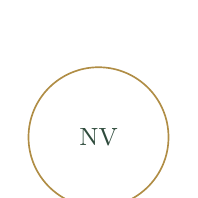
\begin{tikzpicture}
\draw[heritageGold,line width=0.6pt] (0,0) circle (0.35in);
\node[heritageGreen,font=\small] at (0,0) {NV};
\end{tikzpicture}
\end{center}

\end{document}
